\section{Performing Reverse Engineering} \label{sec:performing_reverse_engineering}

\subsection{Level of Granularity}
\paragraph{}
There are many different approaches to start reversing. They can be sorted into two categories, system-level reversing and code-level reversing. They differ according to the level of granularity provided by the analysis, the finest grained ones being not only more complete, but also more complex to realise and understand.

\subsubsection{System Level Reversing}
\paragraph{}
System level reversing is focused on extracting information from a software application through its side effects on the system. As the operating system is the layer of abstraction that prevents software application from having to bother with the dirty details of the underlying hardware, everything has to go through it. Monitoring the effect of a program at a system level can provide a lot of information without the requirement of diving into a pool of assembly lines.

\subsubsection{Code Level Reversing}
\paragraph{}
Code level reversing, as its name suggests, consists of looking at the code (i.e the machine instructions, the Java code, ...) to extract the needed information. Since the code is what instructs the system on what to perform, code level reversing is more general than system level reversing, but the major drawback is that it is significantly harder to perform the former. Offline and live code analysis, two approaches discussed in~\ref{ssec:reversing_approaches}, fit in this category.


\subsection{Reversing Approaches} \label{ssec:reversing_approaches}
\paragraph{}
The process of reversing an executable file can be tackled in many different ways. Depending on what the reverser is looking for, its knowledge, the tools it has in its disposition, and also the legal aspects that could be surrounding the software application under examination, he or she has to find the right approach(es) that suit(s) best that specific need. They will be discussed hereunder.

\subsubsection{Offline Code Analysis}
\paragraph{}
As said before, machine instructions have a one-to-one relationship with assembly instructions, and as a result they can be translated back and forth relatively easily. Offline code analysis consists of translating the machine instructions of an executable file into assembly and inspecting the resulting readable assembly code. The translation from machine instructions to assembly instructions is called disassembly, and it is performed by a disassembler.

\paragraph{}
The main interest of offline code analysis is that the code does not have to be run to be analysed. The reverser can read the generated code to try to find parts that are relevant to his or her analysis.
One drawback is that it does not show the control flow of the program nor the data that is being manipulated as the program advances in the instructions, which makes this approach significantly harder than the others.
It happens that, when an executable file is protected with the right technological protection, offline code analysis is not possible. The reason is that the machine instructions could be obfuscated in such a way that they only appear in their right forms during runtime (or for a certain amount of time during runtime). This will be later explained in Section~\ref{sec:anti_reverse_engineering}.

\subsubsection{Live Code Analysis}
\paragraph{}
This approach also uses the output of a disassembler, but with the addition that it thereafter runs it on what is called a debugger. These tools are used to see how the program evolves as it goes through the instructions, showing the control flow and how the data is being manipulated. This approach is considered easier to perform compared to the offline analysis, but requires the executable file to be run. According to the kind of executable being reversed, a virtual environment could be set up to prevent any damages on the system. More information on virtual environments can be found in Section~\ref{sec:virtual_machines}.

\subsection{Tools}

\subsubsection{Classification Tools} \label{sec:classification_tools}
\paragraph{}
The first thing a reverser has to do when confronted to a binary file is to find out its nature. In the family of Windows's operating systems, most files have extensions that help answering that question but are by no means one hundred percent accurate. An example would be an executable file that ends with the “.exe” extension. Replacing it by one of an image, “.png” for example, won't magically make a picture out of the executable. The example could be extended for any other types of files. A rule of thumb is to never fully trust extensions and to use classification tools that give more than educated guesses. Still, it is wise to not fully rely on the output of a tool, and to corroborate findings amongst many of them if possible. Two of such tools will be briefly presented directly below.

\paragraph{}
The file command can be found in Cygwin\footnote{A Linux-like environment for Windows. See \url{https://www.cygwin.com/}.} as well as many other UNIX/Linux operating systems. Given a sequence of one or more files, it will try to classify them. To do so, it performs three series of tests: file system tests, magic tests, and finally language tests. The command will stop testing as soon as one test yields a match. The file system tests consist of asking the underlying operating system if the file has a special use for it or if it is empty. The magic tests check for numerical or textual values that are unique to specific file types (an example would be the compiled Java classes that are known for having $0xCAFEBABE$ as their first four bytes). Finally, if the two previous series of tests fail, the command will look for human readable text by checking usual character encodings. If nothing can be said, the command will simply say it contains data. An example of use can be found in Figure~\ref{fig:file_command}.

\begin{figure}[!htb]
	\centering
	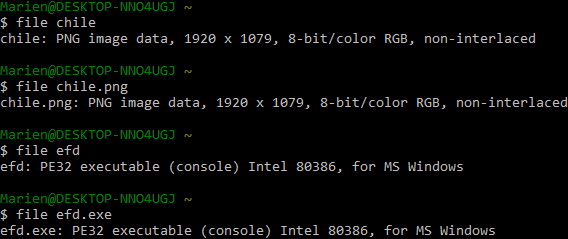
\includegraphics[width=1\textwidth]{reverse_engineering/file_command.png}
	\caption{Using the file command on two pairs of files, with and without their extension.}
	\label{fig:file_command}
\end{figure}

\paragraph{}
Another, more powerful, tool that is also used to identify files is named Detect It Easy\footnote{See \url{http://ntinfo.biz/index.html}.}, or DIE for short. It is specialised for executable file, but it can still identify other file formats. As one can observe in Figure~\ref{fig:detect_it_easy}, it displays the compiler and linker used in the compilation process, the entropy of the file, and much more information related to the structure of the executable. If the file has been packed or obfuscated, the tool can try to find which one has been used by means of specific signatures that can be more sophisticated than magic numbers.

\begin{figure}[!htb]
	\centering
	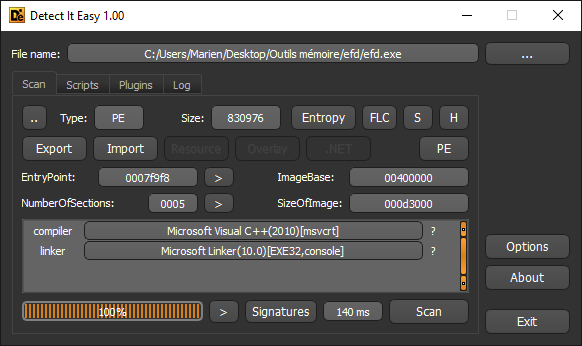
\includegraphics[width=1\textwidth]{reverse_engineering/die.png}
	\caption{Using the Detect It Easy tool to analyse a executable file.}
	\label{fig:detect_it_easy}
\end{figure}

\paragraph{}
There is a myriad of such tools like PEiD\footnote{See \url{http://www.softpedia.com/get/Programming/Packers-Crypters-Protectors/PEiD-updated.shtml}.}, ProtectionID\footnote{See \url{http://pid.gamecopyworld.com/}.}, or even Exeinfo PE\footnote{See \url{http://exeinfo.atwebpages.com/}.}. Those presented are nothing more than two drops in a pool of tools. Some are getting updates more frequently than others, and some are also left to die on the side. What is important is not only to grasp but also to understand how these tools actually work, and to realise that, as the state-of-the-art for tools constantly evolve, it is necessary to keep looking for the sharpest tools.

\subsubsection{Disassemblers} \label{disassembler}
\paragraph{}
Disassemblers are tools that take machine code as input and produce assembly code as output. Since there are many kinds of machine languages, they are usually build specifically to work on a subset of all the languages. To be more precise, disassemblers are built to understand specific ISAs, but also file formats used to wrap code as well as relevant details which can be found in the code that is specific to each operating system. Indeed, machine code intended to be run on an Intel CPU inside a Windows operating system will not be understood by a disassembler built to work on machine code for ARM CPU. 

\paragraph{}
A basic disassembly algorithm is given by Chris Eagle in \textit{The IDA Pro Book}~\cite{eagle2011ida}. It takes machine code as input and it yields assembly language as output:
\begin{enumerate}
	\item Identify where the code is located inside the executable file by parsing the binary according to its executable file format. They usually have an entry point pointer, that is the offset of the first instruction to be decoded and executed.
	\item Fetch the value at the given offset in the file (starting from the entry point) and do a table lookup to match the opcode to its mnemonic. Then decode the operands according to the way the instruction is used.
	\item Once an instruction has been fetched, and any required operands has been decoded, its assembly language equivalent is formatted and output as part of the disassembly listing.
	\item Following the output of an instruction, we need to advance to the next instruction and repeat the previous process until we have disassembled every instructions in the file.
\end{enumerate}

\paragraph{}
Two methods exist to choose which instruction is to be decoded next (step 4): Linear sweep and recursive descend. Linear sweep is the easiest method of the two because it simply decodes instruction directly below the previous one, or in other words, does a linear sweeping until it reaches the end of the code section. The main advantage of this method is that it provides a complete coverage of a program. However, it fails to determine if it is decoding data or code. Indeed, it is possible for data to be in between instructions.

\paragraph{}
Compared to linear sweep, recursive descend avoids the problem of determining whether it is decoding data by using the concept of control flow. When decoding one instruction, it chooses which one is next according to the effect the instruction has on the flow of execution of the program. It is unable to follow indirect code paths (jump, calls) which utilise some kind of lookup table.

\begin{figure}[!htb]
	\centering
	\includegraphics[width=1\textwidth]{reverse_engineering/ia32_disassemble.png}
	\caption{Disassembling a machine code instruction into assembly language. Image inspired by the book \textit{Reversing: Secrets of Reverse Engineering}~\cite{eilam2005reversing}.}
	\label{fig:ia32_disassemble}
\end{figure}

\subsubsection{Decompiler} \label{sec:decompiler}
\begin{framed}
	\begin{definition} 
		A \underline{decompiler}, or reverse compiler, is a program that attempts to perform the inverse process of the compiler; given an executable program compiled in any high-level language, the aim is to produce a high-level language program that performs the same function as the executable program. Thus, the input is machine dependant, and the output is language dependant.
		\begin{flushright}
			\hfill{}{Decompilation of binary programs~\cite{cifuentes1995decompilation}}
		\end{flushright}
	\end{definition}
\end{framed}

\paragraph{}
A fully operational decompiler is the Holy Grail of reverse engineering. If a tool can, from an executable file, generate back the original code that compiles into that executable, there would not be the need for reverse engineers but simply for software engineers. Indeed, if a tool can go backward in the compiling process up to the initial phase, all there is left to do is understanding the source code. Unfortunately, when something is too good to be true, it usually is. The state-of-the-art in decompilation is, generally speaking, not mature enough to provide that silver bullet~\cite{emmerik2004using}.

\paragraph{}
Some of the issues that make decompiling a very complicated task have been identified by Cristina Cifuentes and K.John Gough in their paper titled \textit{Decompilation of Binary Programs}~\cite{cifuentes1995decompilation} and are the following:
\begin{enumerate}
	\item In the Von Neumann architecture, data and instructions are indistinguishable. Because decompilers are working on top of disassembler, and data and instructions can be interspersed, the errors resulting from the disassembly are passed along to the decompiler. Consequently, the decompiling cannot fall back to the original program.
	\item Decompilers are usually made for decompiling executable compiled from a particular programming languages. Compilers and linkers introduce subroutines inside the executable files to, amongst other things, set up the environment before the effective instructions can be processed. These subroutines might not have been written in the programming language for which that particular decompiler is made for. It can also happen that they have been written in assembly, and might not be translatable into a higher level representation.
	\item Not all the operating systems implement mechanisms to share libraries, and so solutions have been created to still allow modular programming. Shared routines from these libraries are instead embedded into the final executable in such a way that coexist with the original program (this is done by the linker). For the reason explained above, the decompiler might not be able to decompile these parts if they are not compiled from the same programming language, or have been written directly in assembly.
\end{enumerate}

\paragraph{}
Nevertheless, viable decompilers exist but with limitations. The Hex-Rays decompiler\footnote{See \url{https://www.hex-rays.com/products/decompiler/}.} is a well known decompiler to a C-like pseudo code text that only works with x86, x64, ARM, and ARM64 targeted executables. It also cannot do type recovery and understanding exception handling. In Listing~\ref{lst:cpp_decompiled_cpp_1} and Listing~\ref{lst:cpp_decompiled_cpp_2}, one can observe a C++ program and its decompiled version after being compiled with GCC\footnote{See \url{https://gcc.gnu.org/}.}. The output of the decompiler is only semantically equivalent as the variable names have changed, the comments have been lost, and the overall structure is different. \\ \\

\noindent\begin{minipage}{.45\textwidth}
	\begin{lstlisting}[caption={Hand written C++ program.}, label={lst:cpp_decompiled_cpp_1}, frame=tlrb, language=C++]
int fact(int n) {
	// A very useful comment
	if (n <= 0)
		return 1;
	return n * fact(n - 1);
}
	\end{lstlisting}
\end{minipage}\hfill
\begin{minipage}{.45\textwidth}
	\begin{lstlisting}[caption={Output of the Hex-Rays Decompiler applied to the compiled version of the code found in Listing~\ref{lst:cpp_decompiled_cpp_1}.}, label={lst:cpp_decompiled_cpp_2}, frame=tlrb, language=C++]
int __cdecl fact(int n)
{
	int result; // eax@2
	
	if ( n > 0 )
		result = n * fact(n - 1);
	else
		result = 1;
	return result;
}
	\end{lstlisting}
\end{minipage}           

\paragraph{}
It is worth noticing that some programming languages such as Java and C\# have decompilers which yield outputs that are very close to the original programs. This phenomenon can be explained by how these programming languages are compiled. They both use intermediary representations in which the ISA is still abstracted away, usually with the intent of staying platform independent. As a result, many of the information that would usually be removed by a compiler that compiles into machine code stays in the file until runtime. Obviously, once the executable starts being executed, the Java or C\# compiler has to finish the job so that the CPU can understand the instructions. An example of decompiler program obtained with JD-GUI\footnote{See \url{http://jd.benow.ca/}.} can be observed in Listing~\ref{lst:java_decompiled_java_1} and Listing~\ref{lst:java_decompiled_java_2}. In comparison with C++ code,  variable names are kept intact as well as the structure of the method. Still, the commentaries are lost as they serve no real purpose outside the development phases. \\ \\

\noindent\begin{minipage}{.45\textwidth}
	\begin{lstlisting}[caption={Hand written Java program.}, label={lst:java_decompiled_java_1}, frame=tlrb, language=Java]
/**
* For a given name, generate
* a greeting string message.
* @param name
* @return the string
*/
String greets(String name) {
	String str = "Welcome, ";
	str += name + ".";
	return str;     
}
	\end{lstlisting}
\end{minipage}\hfill
\begin{minipage}{.45\textwidth}
	\begin{lstlisting}[caption={Output of the JD-GUI decompiler applied to the partially compiled version of that code found in Listing~\ref{lst:java_decompiled_java_1}.}, label={lst:java_decompiled_java_2}, frame=tlrb, language=Java]
String greets(String name)
{
	String str = "Welcome, ";
	str = str + name + ".";
	return str;
}
	\end{lstlisting}
\end{minipage}

\subsubsection{Debuggers}
\paragraph{}
Debuggers are tools that fit in the live code analysis category. They are used to observe and control the internal state and execution of a running process~\cite{sikorski2012practical}. Compared to disassemblers, they require the executable file being analysed to be run, but at the same time, they provide more detailed information about what is happening inside such as a real time visualisation of the registers and the system memory.

\paragraph{}
Breakpoints are used to pause the execution of a process and so, it is a mandatory feature for debuggers. Without the ability to pause a process's execution, it is impossible to observe its state changing, which is the point of a debugger. There are two kinds of breakpoints, software and hardware breakpoints. As their names suggest, the software breakpoints are implemented by the software, and the hardware ones, by the processor. Software breakpoints are implemented by replacing the instructions where the process has to stop by either a system call or an invalid instruction which will cause the debugger to take over. Hardware breakpoints are implemented on x86 architecture by special debugging registers that contain addresses. Once the process accesses one of these addresses, it will be paused by the processor, and the debugger will regain the control. Hardware breakpoints are specially useful when one wants to see when a piece of data is being accessed (a global variable, for example).

\paragraph{}
A debugger can either be attached to an existing process or start a new one from a selected application, being source-level or assembly-level, and finally be run in user or kernel mode. These distinctions will be discussed hereunder.

\paragraph{}
If one wants to analyse a running process, it has to attach a debugger to it (a procedure that has to be done with the support of the operating system). By doing so, all the threads that compose that process will be paused, and the reverse engineer will be free to do whatever he or she wants. This can be useful when one wants to debug a process after it has been running for awhile or to analyse the changes a malware could have done to it. Debuggers also allow to start a new process by selecting an executable file. In that case, the process will be paused in its entry point for the reverser to start doing its job.

\paragraph{}
Assembly-level debuggers are built on top of a disassembler and so, allows reverse engineers to debug an executable file at the level of the assembly instructions. Code-level debuggers are usually found in IDE (short for Integrated Development Environment) which are environment for programmers to be more productive when developing applications. They allow to debug directly at the source code level, which does not expose the developers to assembly instructions. In this work, the word debugger means assembly-level debugger.

\paragraph{}
As said before, the x86 ISA provides ring levels for a better separation between the operating system and the programs belonging to the users. A user mode debugger will, as its name suggests, be running in user mode, and so, will not be capable of debugging kernel level application. A kernel mode debugger can also debug user level application, but with an extended control over the operating system, as well as debugging kernel level application such as the operating system itself. To be noted that it is usually necessary to have two systems for performing kernel level debugging as to put a breakpoint in a kernel will freeze one of the two. 

\subsubsection{Strings Detecting Tools}
\paragraph{}
Contrary to debuggers and disassemblers, string detecting tools do not need to have any knowledge about the structure of an analysed file, they only have to be aware of what constitutes a string. As such, these tools can be used on virtually any kind of files. The listing they produce can be useful to get a broad idea of the functionality of a program. An example would be extracting error messages that could be stored inside an executable file for they can be informative about the purpose of the application.

\paragraph{}
In a computer's memory, characters are encoded using encodings such as UTF-8, which supports all characters defined by Unicode or even ASCII, short for American Standard Code for Information Interchange, that only handles a subset of Unicode. The strings detection tools have to be aware of these different representations to discriminate a string from the rest of what composes a file. They can also be subject to false positive. Indeed a sequence of bytes could very well match one of the encoding while being something unrelated. 

\paragraph{}
Microsoft provides a tool named Strings free of charges on its website\footnote{\url{https://technet.microsoft.com/en-us/sysinternals/bb897439}}. It can display ASCII and Unicode\footnote{It does not make too much sense since Unicode is not an encoding, but that is how they advertise the tool.} encoded strings with their offset (address), and it allows to filter srings that are below a certain size (three by default). Moreover, one can refine the search by specifying a starting and ending offset in the file to be analysed. An example of utilisation can be found in Figure~\ref{fig:strings_in_action}. 

\begin{figure}[!htb]
	\begin{minipage}[b]{0.4\textwidth}
		\centering
		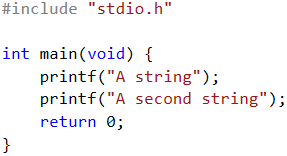
\includegraphics[width=1\textwidth]{reverse_engineering/strings_c_code.png}
	\end{minipage}
	\hfill
	\begin{minipage}[b]{0.4\textwidth}
		\centering
		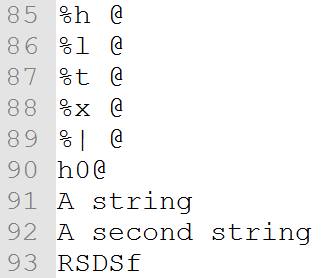
\includegraphics[width=0.7\textwidth]{reverse_engineering/strings_output.png}
	\end{minipage}
	\caption{On the left, a program written in c that was later compiled in Visual Studio 2015. On the right, the listing of strings applied to the executable file produced by the program on the right. False positives are usually easy to detect as they do not mean anything.}
	\label{fig:strings_in_action}
\end{figure}


\subsubsection{PE Analysis Tools}
\paragraph{}
The Portable Executable, or PE for short, is a file format used to structure executable files, object code, and DLLs on operating systems from the Windows NT family. As explained in Section~\ref{sec:executable_file_format}, this structure contains the machine code as well as the meta data that are used by the operating system to load and manage the executable file. The meta data can provide a reverse engineer with information about the type of the file, the sections it contains, the debugging information left by the compiler, the resources such an icon and the manifest file, the imported functions, the exported functions, the relocation table, and the list goes on. Clearly, tools allowing to see these meta data are of great use. Hereunder it will be presented PEBrowse Professional\footnote{\url{http://www.smidgeonsoft.prohosting.com/pebrowse-pro-file-viewer.html}}, but it is by no means the only tool able to provide such functionalities.

%---------------- Corrected up to here

\begin{figure}[!htb]
	\centering
	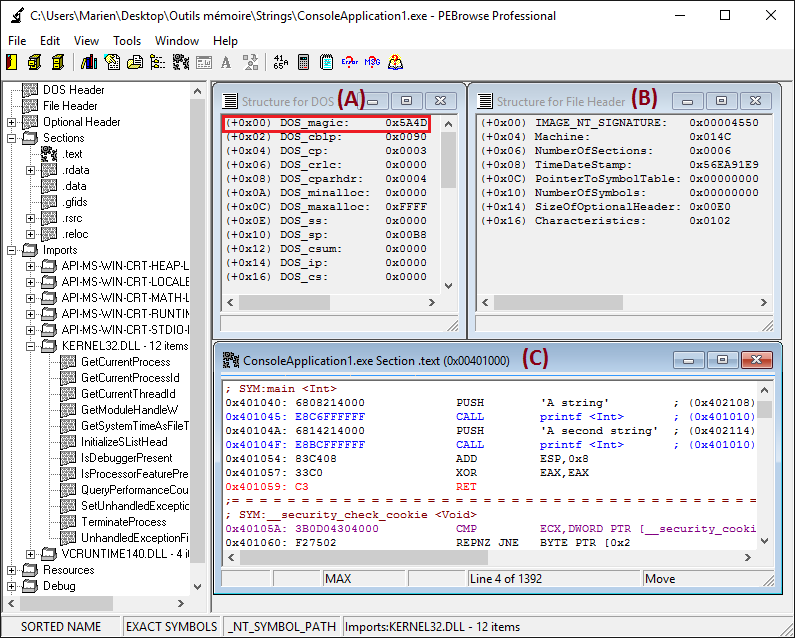
\includegraphics[width=1\textwidth]{reverse_engineering/pebrowse_professional_annotated.png}
	\caption{Screen shot of PEBrowse Professional used on a simple executable.}
	\label{fig:pebrowse_professional}
\end{figure}

\paragraph{}
As one can see in Figure~\ref{fig:pebrowse_professional}, the interface is divided into two parts. The left column contains the names of the components that compose the PE structure and the right part contains detailed view of these components. They are opened through the contextual menu that appears once an element of the left column is right clicked. From top to bottom, the left column contains:
\begin{itemize}
	\item \textbf{DOS Header}: For compatibility reasons, a valid MS-DOS program is the first thing one can find upon opening a file which uses the PE format. A partial view of the header can be observed on \textbf{(A)}. One might have noticed the magic number $0x4D5A$ (or MZ) in the red square, which is used by the file command discussed in Section~\ref{sec:classification_tools}.
	\item \textbf{File Header}: It contains information about the file, for instance, for  which system it was compiled, the number of sections, the timestamp at which the header was generated, whether it is an executable file or a DLL, and some other minor information. A partial view of the header can be observed in \textbf{(B)}.
	\item \textbf{Optional Header}: This header is not optional. Inside it can be found the version of the linker used to make the file, the entry point of the program, a checksum of the file, and much more information.
	\item \textbf{Sections}: As the name suggests, this part contains the different sections that compose a program. “.text” contains the machine instructions, “.data” contains global data, “.rdata” has the same use with the difference that it is read-only, “.reloc” contains the relocation table, “.rsrc” contains the resources of the program such as the manifest that tells the operating system if an elevation of privileges is necessary. The tool also contains a disassembler, and a view of its ouput can be observed in \textbf{(C)}.
	\item \textbf{Imports}: Here it can be found the DLLs which export functions used by the file, as well as the function names.
	\item \textbf{Resources}: It is a shortcut to get to the resources stored in the file.
	\item \textbf{Debug}: It is a shortcut to get to the debugging information which could come with the file.
\end{itemize}

\paragraph{}
The PE format is a very complex subject. For more information on the topic, see the article of Matt Pietrek published in the MSDN Magazine~\cite{pietrek2002inside}.


\subsubsection{Tracing Tools}
\paragraph{}
Tracing is a technique that allows someone to understand what is happening in a software system\footnote{A software system is the set of programs which are running on a specific hardware system.} by tracing the execution of its processes. A tool able to perform tracing is called a tracer. An interesting property of this family of tools is that, they do not require the reverser to dive into assembly code. Indeed, their only purpose is to record the occurrences of certain events that are triggered by the probes they disseminate. These events can either be printed on the screen or saved in a file for further analysis, and the probes can be installed inside the operating system's kernel or any software application.

\paragraph{}
It is important to differentiate logging from tracing for they do not operate at the same level of complexity. On one hand, logging is used for high level analysis of infrequent events such as networking failure or database accesses. On the other hand, tracing is used at a very low level to monitor events such as system calls and library calls.

\paragraph{}
Strace\footnote{See \url{http://man.he.net/man1/strace}.} is an open source tracer developed for Linux and provided in most distribution to intercepts system calls made by processes as well as signals received by processes, with the support of the kernel. It can also trace the child processes as they are created by the main process, trace interactions with the kernel, and provide options to specify what kind of system calls and signals must be logged. Ltrace\footnote{See \url{http://man.he.net/man1/ltrace}.} is also a tracer but with the particularity that it can only log calls made to shared libraries. It then does not require support from the kernel and provides more readable outputs. In Figure~\ref{fig:ltrace} can be observed the output of ltrace on a simple “hello world” program.

\begin{figure}[!htb]
	\centering
	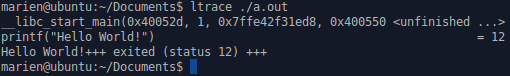
\includegraphics[width=1\textwidth]{reverse_engineering/ltrace.png}
	\caption{Output of ltrace on a simple “hello world” program.}
	\label{fig:ltrace}
\end{figure}

\subsubsection{Monitoring Tools}
\paragraph{}
Monitoring tools are similar to tracing tools for they provide information about the behaviour of processes. The difference is that they yield outputs that are more high level than, for example, a listing of all the system calls made by a specific process. Because communication with the operating system is necessary to make use of a computer, and since tracers are used to analyse these exchanges, monitoring tools are usually built on top of tracers. As it might be expected, they do not require the reverser to work at the level of assembly code either. 

\paragraph{}
The Windows Sysinternals Suite\footnote{See \url{https://technet.microsoft.com/en-us/sysinternals/bb842062.aspx}.} is a collection of tools made freely available by Microsoft to help with managing, troubleshooting and diagnosing Windows systems and applications. Some of its tools will be discussed hereunder.
\begin{itemize}
	\item \textbf{Handle}: For every process in the system, this tool gives its list of open handles. A handle is a reference to an open file, which can also be a registry key.
	\item \textbf{ListDLLs}: As its name suggests, this tool is used to list all the DLLs that are loaded into a process.
	\item \textbf{Procmon}: Short for Process Monitor, it is a combination of legacy tools called respectively Filemon and Regmon (File and Registry Monitor). It displays in real time file system, registry and process/thread activity while providing very useful filtering capabilities.
	\item \textbf{TCPView}: This tool lists all the TCP and UDP connections made by the processes of the system. For each connection, it is displayed the protocol, local and remote addresses, local and remote ports, the state of the connection, and statistics about the exchanged packets.
	\item \textbf{Sysmon}: Short for System Monitor, it is a service and device driver that does not have to be manually restarted across reboots. It logs information about system activities such as process creation, changes to file, and network connection.
	\item \textbf{Procexp}: Short for Process Explorer, it is a more complete version of the task manager provided by default on Windows. It shows the currently active processes, and for each of them, the open handles, the loaded DLLs, and the memory mapped files, while providing the other functionalities found in the original task manager. Compared to the other tools discussed above that provide the same capabilities, procexp has an intuitive graphical interface that makes it easier for these activities to be monitored.
\end{itemize}

\subsubsection{Virtual Machines} \label{sec:virtual_machines}
\paragraph{}
A virtual machine could be seen as a computer running inside another computer. The host computer is usually a concrete computer that has a CPU which provides functionalities for virtualisation, and the guest computer is the computer running on top of the host computer. This can be observed in Figure~\ref{fig:virtual_machine}, where normal applications, such as a browser, are seen sharing the system with a virtual machine.

\begin{figure}[!htb]
	\centering
	\includegraphics[width=0.6\textwidth]{reverse_engineering/virtual_machine.png}
	\caption{A virtual machine living in an operating system. Image inspired by the book \textit{Practical Malware Analysis: The Hands-On Guide to Dissecting Malicious Software}~\cite{sikorski2012practical}.}
	\label{fig:virtual_machine}
\end{figure}

\paragraph{}
A virtual machine can be useful depending on the kind of executable that is being analysed. If someone running on Windows system wants to perform live debugging on an executable compiled for Linux, he or she might want to make use of this technique. Another situation that justifies the need of virtualisation is when dealing with malware applications. Because these programs can have disastrous effects on the system it is being analysed on, and on the neighbouring systems as well, it is greatly advised to isolate that system from the rest of the world.

\paragraph{}
An interesting functionality of virtual machines is the possibility to save the current state of a virtualised system to restore it later. The saved state is usually called a snapshot. An example of how this technology could be used would be to take a snapshot of a clean system, run a malware, analyse the damages/changes it has done, and then finally roll-back to the clean state to analyse another malware.

\paragraph{} 
VMware Workstation\footnote{A virtualisation sofware, see \url{https://www.vmware.com/}.} provides another feature called record/replay that can be useful to speed up debugging sessions. Once activated, VMware will start recording through its virtualisation layer the complete execution behaviour of the applications being executed inside the virtual machine. This recording allows the machine to go back in time to replay the same exact behaviour, over and over again~\cite{vmware_record_replay}. Conceptually, it is equivalent to a system wide “undo”. If, for example, a reverse engineer enters a function that never ends, he or she can either restart the debugging session or replay the recording until a little bit before jumping into that function.

\subsubsection{Memory Scanning Tools}
\paragraph{}
These tools are used to scan the memory of a process for specific variables using filtering rules that provide an iterative refinement. Examples are often worth a thousand words, so let's explore a simple scenario. One could find itself stuck in a level of a very challenging video game. Instead of applying the well-known fail and retry approach, the lazy gamer can use a memory scanning tool to identify variables of interest such as the life or score counter with the intent of applying beneficial modifications.

\paragraph{}
In our previous scenario, the challenge of beating the game has been replaced by finding these variables. To do so, the tool has to first identify all the possible variables present in the process, and then to provide the possibility to rescan for specific changes in these variables. Those who did not changed in that specific way are filtered out. When the player takes damage, the variable holding the amount of life left will in most case decrease. One can try to find its location by taking damages, scanning for decreasing variables, and repeating these operations until one variable is left.

\paragraph{}
When using a Linux system, one can use scanmem\footnote{See \url{http://linux.die.net/man/1/scanmem}.}. It provides a means to both locate and modify a variable in a running process, but no graphical interface is provided directly. On Windows, there is the famous Cheat Engine\footnote{See \url{http://www.cheatengine.org/}.} that also provides a means to locate and modify variables, but also comes with a useful graphical interface that makes the research easier, and consequently faster. It can be observed in Figure~\ref{fig:cheat_engine}. 

\begin{figure}[!htb]
	\centering
	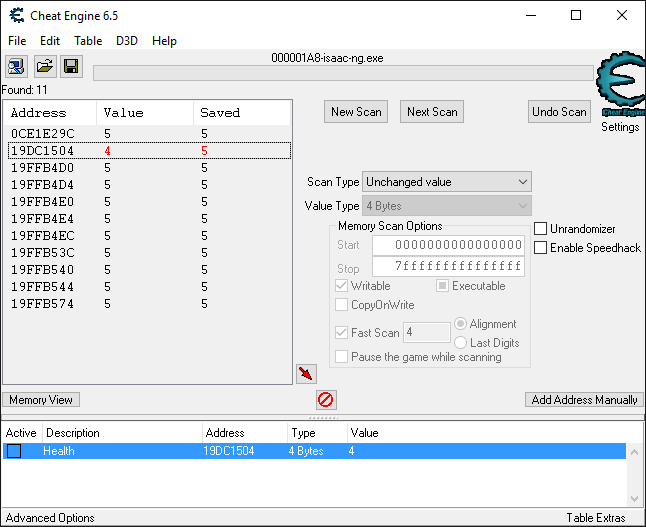
\includegraphics[width=1\textwidth]{reverse_engineering/cheat_engine.png}
	\caption{Cheat Engine used on The Binding of Isaac: Rebirth.}
	\label{fig:cheat_engine}
\end{figure}

\subsubsection{Hex Editors}
\paragraph{}
Hex editors are to programs what text editors are to text files. They provide a means to edit files of any kind through their hexadecimal representations instead of the textual one, if it exists. It can be observed in Figure~\ref{fig:hex_editor} HxD\footnote{See \url{https://mh-nexus.de/en/hxd/}.} tool, a free hex editor running on all versions of Windows starting from 95. The main window contains three columns that can be identified by the spaces that separate them. On the left, one can see the starting addresses of the 16 byte arrays that are found in the middle column. On top of that column are given the offsets that have to be added to the array address to get the address of each byte. The right column simply shows a textual representation of the bytes using a specific encoding. Here, ANSI is used.

\begin{figure}[!htb]
	\centering
	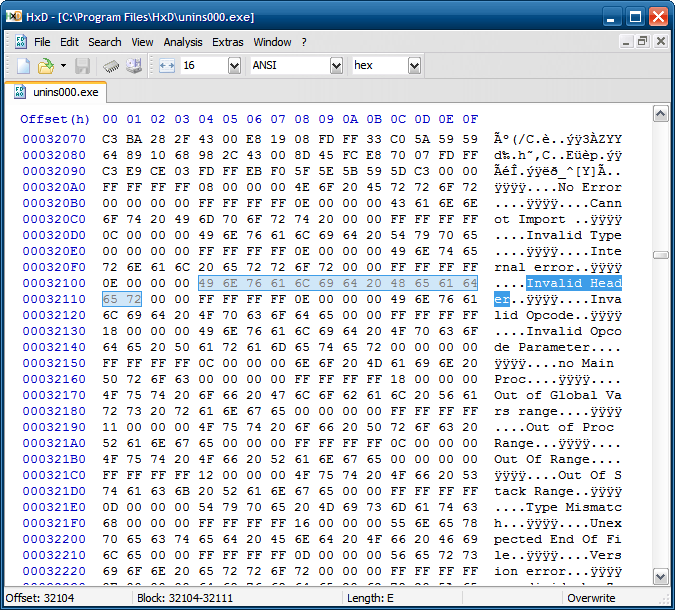
\includegraphics[width=1\textwidth]{reverse_engineering/hex_editor.png}
	\caption{HxD displaying the uninstall executable file of HxD.}
	\label{fig:hex_editor}
\end{figure}

\subsubsection{Visualisation Tools}
\paragraph{}
Given enough time and resources (such as man power and tools), any reverse engineer can potentially extract what he or she is looking for from a binary file. Life being what it is, ephemeral, we all have a limited amount of both. Visualisation tools shine at providing information about the overall perspective of a file in a way that requires little to no time to be understood. Consequently, it can greatly speed up the reversing process. In this section, two kinds of tools will be discussed. The first one does not care about the structural representation of the file being analysed, whereas the second one does.

\paragraph{}
The entropy measures a system's disorder. The higher is the value, the less ordered is the system. A sequence of the same characters has then little entropy, whereas a sequence made of all the characters that can exist on that system will have the highest entropy. Aldo Cortesi, a New Zealander security consultant had the idea of computing the entropy of a file using the Shannon entropy~\cite{shannon1951prediction} over a sliding window to make the task of finding compressed data/cryptographic material inside executable files easier. They indeed have higher entropy levels than regular data such as strings and assembly code. To display the information in an intuitive way, he used the Hilbert curve~\cite{voorhies1991space} for it gives a mapping between one dimensional and two dimensional spaces that preserves locality. His tool\footnote{See \url{http://binvis.io/}.} can be used online, directly on his website. In Figure~\ref{fig:entropy}, it can be observed the result of applying this analysis to TCPview. To be noted that entropy is not the only information that can be displayed with that tool. The byteclass colour scheme gives a blue colour for character, and different colours for non textual data, as seen in Figure~\ref{fig:byteclass}. There are two other schemes at the time of writing, one can refer to the author's website for more information.

\begin{figure}
	\begin{minipage}[b]{0.4\textwidth}
		\centering
		
\includegraphics[width=0.3\textwidth]{reverse_engineering/tcpview_entropy.png}
		\caption{The closer the colour is to pink, the more entropy that part has.}
		\label{fig:entropy}
	\end{minipage}
	\hfill
	\begin{minipage}[b]{0.4\textwidth}
		\centering
		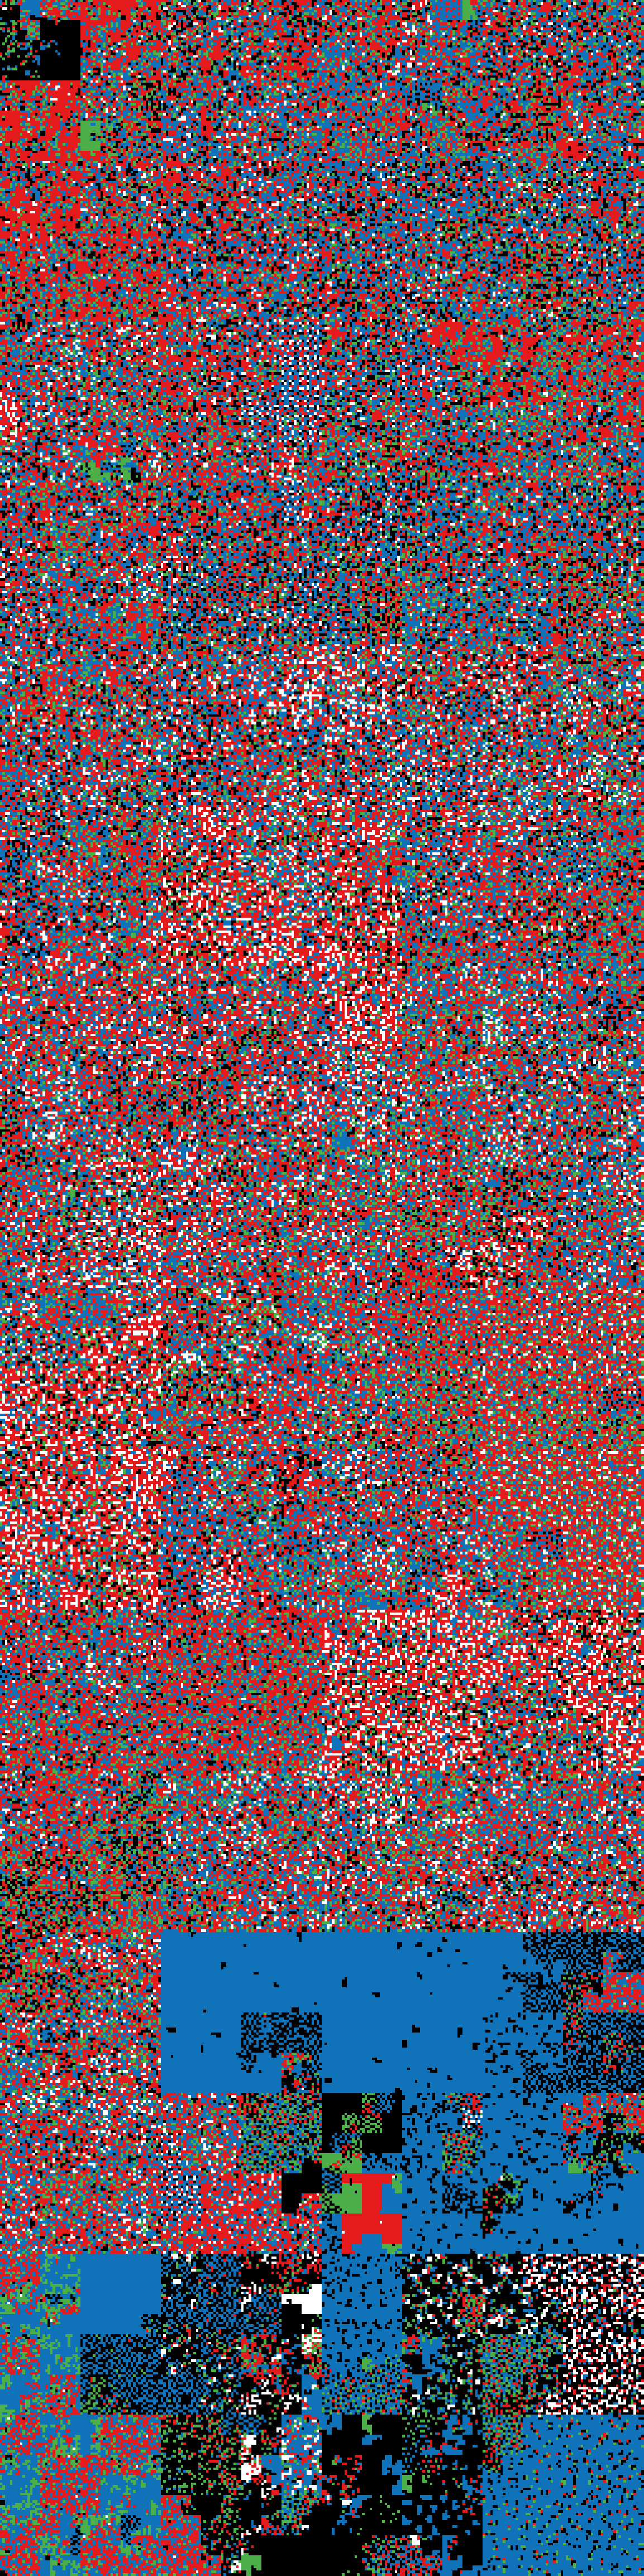
\includegraphics[width=0.3\textwidth]{reverse_engineering/tcpview_byteclass.png}
		\caption{Blue represent characters, black represents 0x00, white 0xff, green and red is the rest.}
		\label{fig:byteclass}
	\end{minipage}
\end{figure}


\paragraph{}
A control flow graph (CFG for short) is a representation of all the paths a program can take during its execution. For example, conditional statements such as an $if–then–else$ split the path of execution at least into two trails. A CFG is very useful as it shows these branches in a directed graph and gives insight on how the program can unfold. A trained reverser can even easily identify specific constructs simply by looking at the structure of the graph. A CFG generated with IDA\footnote{A disassembler and debugger which provide a plethora of functionalities. See \url{http://www.hex-rays.com/}.} can be observed in Figure~\ref{fig:control_flow_graph}. A creative reader could find the totally useless but quite remarkable tricks to turn a control flow graph into a grey scale image interesting. This idea has been developed by Christopher Domas with the goal of deterring potential reverse engineers by “crushing their souls”\footnote{See his DEF CON presentation: \url{https://github.com/xoreaxeaxeax/REpsych}.}.

\begin{figure}
	\centering
	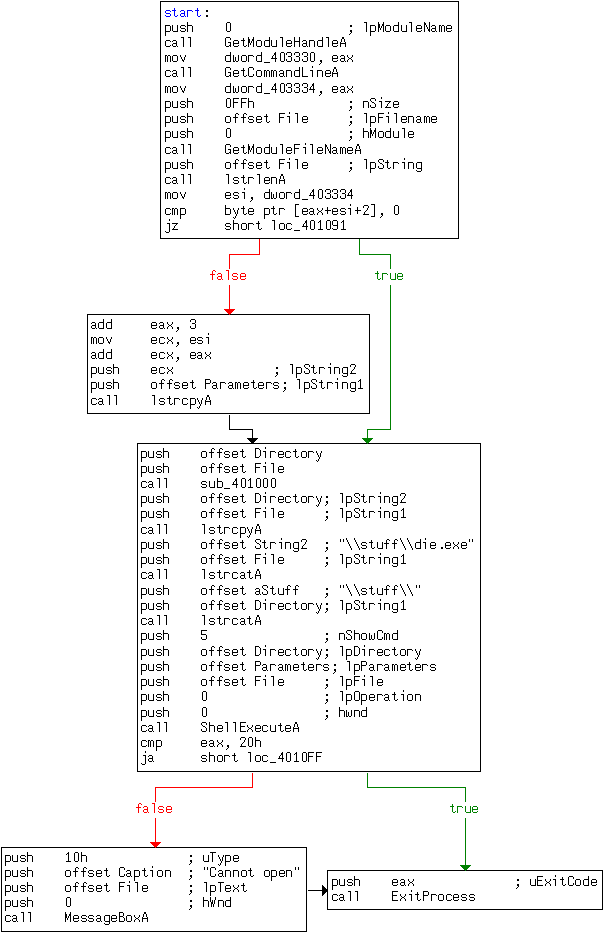
\includegraphics[width=0.8\textwidth]{reverse_engineering/control_flow_graph.png}
	\caption{A control flow graph generated by IDA. If-then-else constructs are easily identifiable.}
	\label{fig:control_flow_graph}
\end{figure}

\paragraph{}
Another more useful work done by Christopher Domas is the interactive binary visualisation tool ..cantor.dust..\footnote{See \url{https://sites.google.com/site/xxcantorxdustxx/visual-re}.} presented in various security conferences. It uses the ideas of Aldo Cortesi and Gregory Conti~\cite{conti2008visual} to visualise information in a graphical way, but also introduces an automated mechanism for classifying different regions of a file according to the type of information they contain using statistical methods. The annotated output can be observed in Figure~\ref{fig:cantor_dust}. Sadly, at the time of writing, the tool has not been released to the public and the author has been silent on the subject for a rather long period of time. For more information, one should watch one of his presentations entitled “The Future of RE Dynamic Binary Visualization”.

\begin{figure}[!htb]
	\centering
	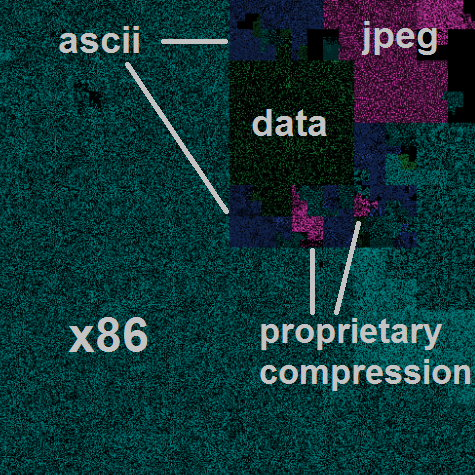
\includegraphics[width=0.45\textwidth]{reverse_engineering/cantor_dust.png}
	\caption{Annotated output of ..cantor.dust.. Image from the presentation.}
	\label{fig:cantor_dust}
\end{figure}